\section{Gelijktijdigheid: Deadlocks en uithongering}

\subsection{Beginselen van deadlock}

Een \textbf{deadlock} is een permanente blokkering van processen die met elkaar wedijveren om bronnen of die met elkaar communiceren. Er is geen efficiënte manier om een deadlock op te lossen.

\begin{figure}[htp]
    \centering
            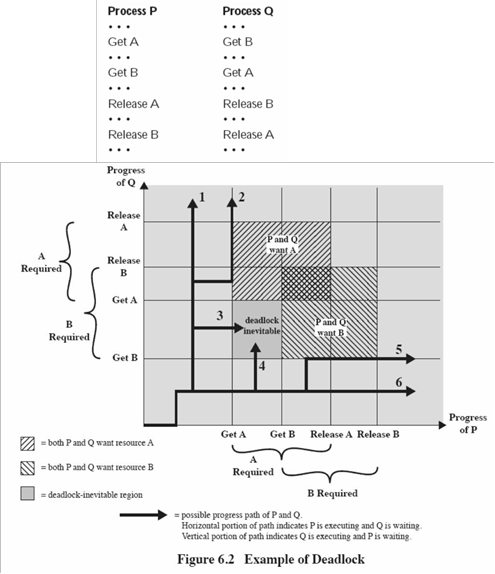
\includegraphics[width=4in]{img/deadlock.png}
        \caption{Voorbeeld deadlock}
    \label{fig:Voorbeeld deadlock}
\end{figure}

\begin{figure}[htp]
    \centering
            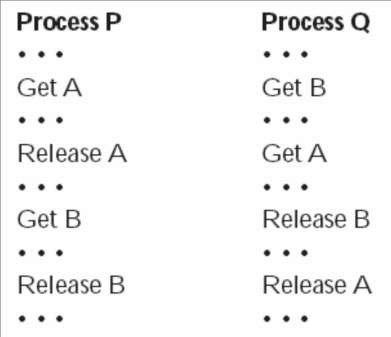
\includegraphics[width=4in]{img/processen.png}
        \caption{Voorbeeld deadlock}
    \label{fig:Voorbeeld deadlock}
\end{figure}


\begin{figure}[htp]
    \centering
            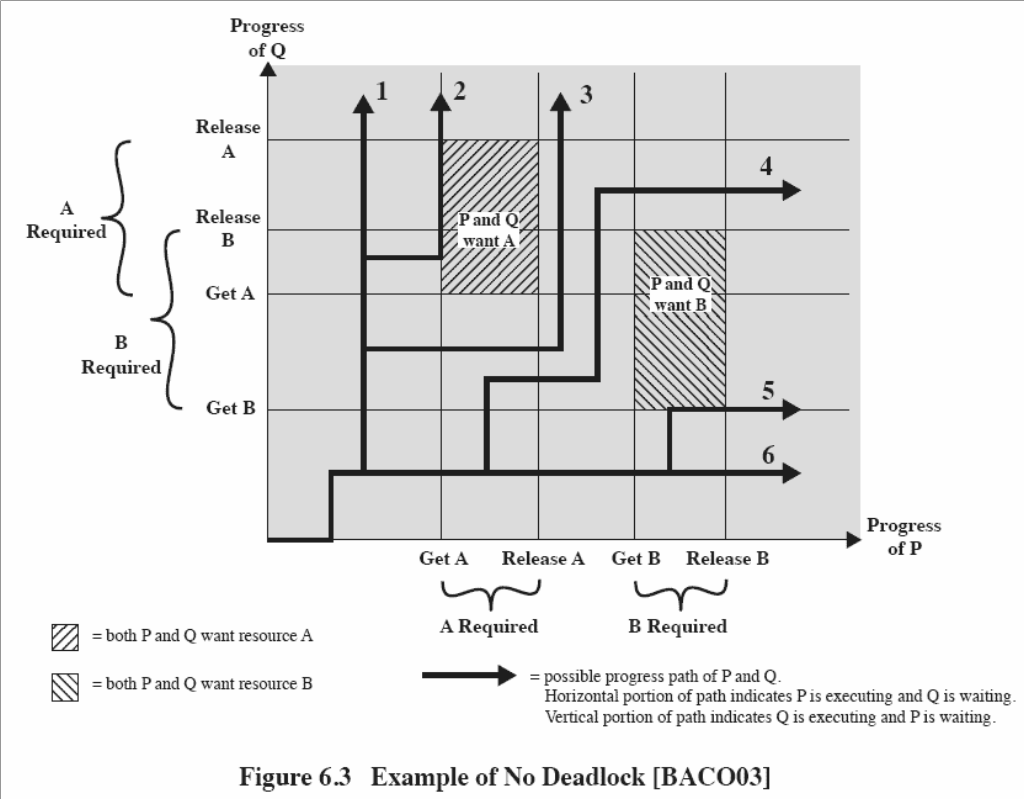
\includegraphics[width=4in]{img/nodeadlock.png}
        \caption{Voorbeeld geen deadlock}
    \label{fig:Voorbeeld geen deadlock}
\end{figure}


\subsubsection{Herbruikbare hulpbronnen}

Er zijn 2 soorten bronnen:

\begin{itemize}
\item Herbruikbare bronnen (reusable resources): deze kan veilig gebruikt worden door 1 proces na het gebruik ervan is de bron nog steeds beschikbaar.
\item Verbruikbare bronnen (consumable resources): Deze bronnen worden aangemaakt en terug vernietigd.
\end{itemize}

Voorbeelden van herbruikbare bronnen:

\begin{itemize}
\item Processors
\item I/O-kanalen
\item Hoofdgeheugen en secundair geheugen
\item Apparaten
\item Gegevensstructuren, bv. Bestanden
\item Databases
\item Semaforen
\end{itemize}

\begin{figure}[htp]
    \centering
            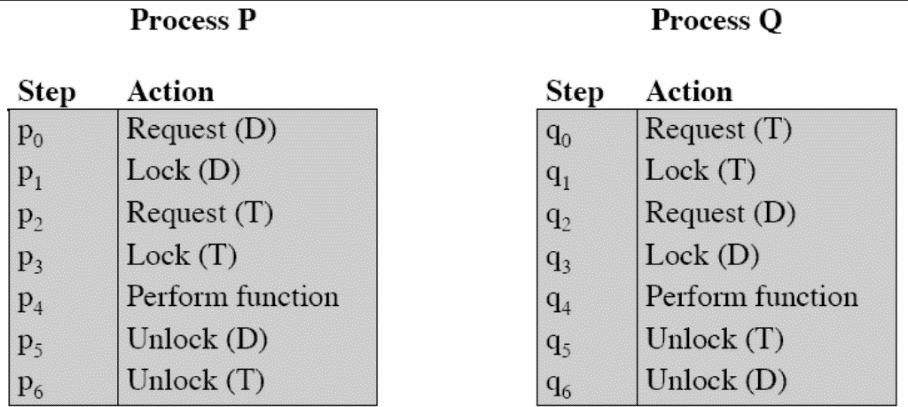
\includegraphics[width=4in]{img/processenherbruikbaar.png}
        \caption{Voorbeeld geen deadlock}
    \label{fig:Voorbeeld geen deadlock}
\end{figure}

\subsubsubsection{Verbruikbare bronnen}
Voorbeelden van verbruikbare bronnen:

\begin{itemize}
\item Interrupts
\item Signalen
\item Berichten
\item Gegevens in I/O buffers
\end{itemize}

Voorbeeld van een deadlock met verbruikbare bronnen: P1 wacht op een bericht van P2 om naar P2 te versturen terwijl P2 wacht op een bericht van P1 om naar P1 te versturen.

=> een deadlock treedt op als het ontvangen blokkerend is

\begin{figure}[htp]
    \centering
            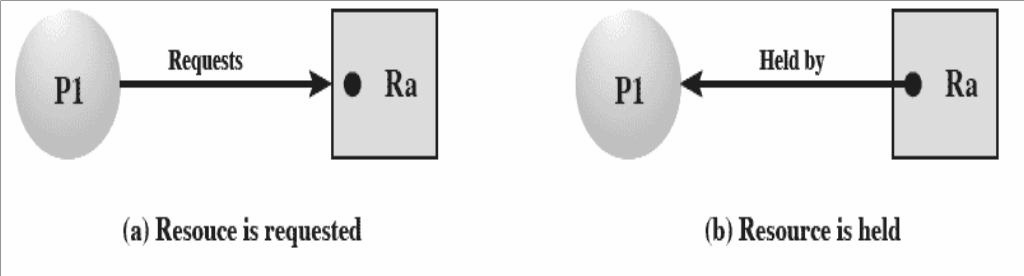
\includegraphics[width=4in]{img/Brontoewijzingsschemas.png}
        \caption{Voorbeeld geen deadlock}
    \label{fig:Voorbeeld geen deadlock}
\end{figure}

Een punt is een voorstelling van een bron, hierboven is er van elke bron maar 1 instantie een proces vraagt om een bron maar die nog niet toegewezen, pas wanneer er een pijl van een bron naar een proces gaat is de bron toegewezen aan dat proces.

\subsubsection{Condities voor een mogelijke deadlock}

\begin{itemize}
\item Wederzijdse uitsluiting: een bron mag maar aan 1 proces gelijktijdig worden toegewezen
\item Vasthouden en wachten: een proces mag een bron vasthouden terwijl het wacht op de toewijzing van andere bronnen
\item Geen preëmptieve onderbreking: een bron kan niet zomaar worden afgenomen van een proces dat de bron vasthoudt
\end{itemize}

Hierboven staan de voorwaarden voor een mogelijke deadlock, om een echte deadlock te krijgen moet er nog aan een extra conditie worden voldaan:

\begin{itemize}
\item Cirkelvormig wachten: een ketting van wachtende processen waarbij de processen wachten op het vrijkomen van een bron dat een ander proces vasthoudt.
\end{itemize}

Er zijn drie strategieën om te gaan met een deadlock: voorkomen, vermijden en detecteren

Voorbeelden van deadlocks:



\begin{figure}[htp]
    \centering
            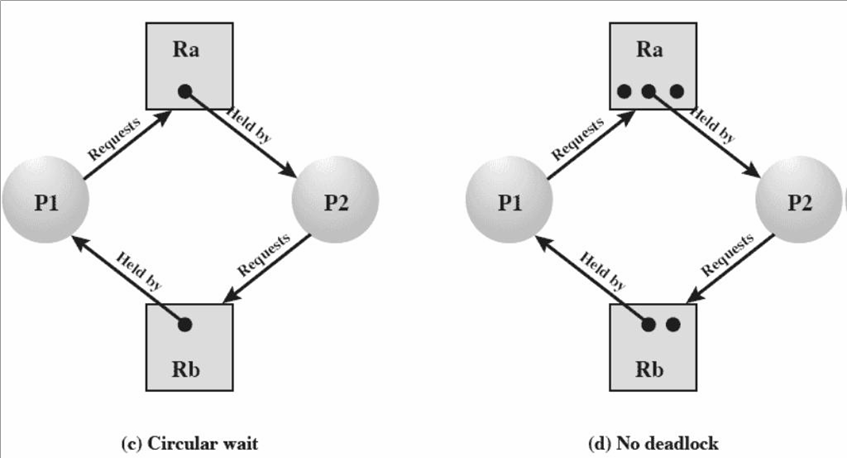
\includegraphics[width=4in]{img/deadlockexamples.png}
        \caption{Voorbeeld geen deadlock}
    \label{fig:Voorbeeld geen deadlock}
\end{figure}

\begin{figure}[htp]
    \centering
            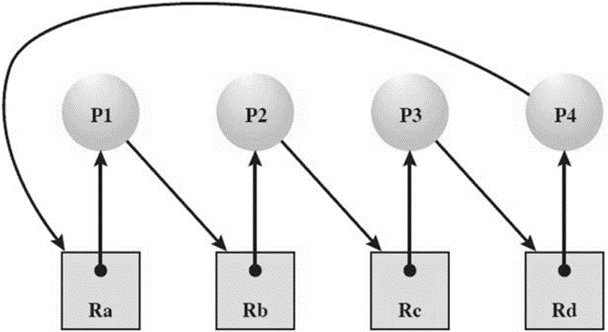
\includegraphics[width=4in]{img/deadlockomgaan.png}
        \caption{Voorbeeld geen deadlock}
    \label{fig:Voorbeeld geen deadlock}
\end{figure}

Je kan op drie manieren omgaan met deadlocks:

\begin{itemize}
    \item Deadlocks voorkomen
    \item Deadlocks vermijden
    \item Deadlocks opsporen
\end{itemize}

